%\frameT{Outline}{
%  \begin{enumerate}
%    {\transparent{0.2} \item The languages of P-trees, PLP-trees, and LP-trees}
%    {\transparent{0.2} \item Learning preference models in case of PLP-trees}
%    \item Reasoning with preferences:
%      \begin{itemize}
%        \item Preference optimization in case of P-trees
%        {\transparent{0.2} \item Computing winners and ``strong" candidates when votes are LP-trees}
%        {\transparent{0.2} \item Application in trip planning}
%      \end{itemize}
%    {\transparent{0.2} \item Future research directions}
%  \end{enumerate}
%}
%
%\frameT{Computational Complexity Results for P-trees}{
% Dominance-testing ({\sc DomTest}): $o_1 \succ_T o_2$?\\
% Optimality-testing ({\sc OptTest}): $o$ optimal w.r.t $T$?\\
% Optimality-with-property ({\sc OptProp}): is there optimal $o$ 
% with property $\alpha$?
%
% \begin{enumerate}
%   \item {\sc DomTest}$\;\in P$
%   \item {\sc OptTest}$\;\in \coNP$-complete:
%     \begin{itemize}
%       \item The complement problem is reduced from the SAT problem.
%     \end{itemize}
%   \item {\sc OptProp}$\;\in \deltap{2}$-complete:
%     \begin{itemize}
%       \item The problem is reduced from the Maximum Satisfying Assignment (MSA) problem. 
%     \end{itemize}
% \end{enumerate}
%}

\frameT{Outline}{
  \begin{enumerate}
    {\transparent{0.2} \item The languages of PLP-trees and LP-trees}
    {\transparent{0.2} \item Learning preference models in case of PLP-trees}
    \item Reasoning with preferences:
      \begin{itemize}
        \item Computing winners and ``strong" candidates when votes are LP-trees
        {\transparent{0.2} \item Application in trip planning}
      \end{itemize}
    {\transparent{0.2} \item Future research directions}
  \end{enumerate}
}

\frameT{Positional Scoring Rules}
{
	\begin{itemize}
		\item $k$-approval: ($1,\ldots,1,0,\ldots,0$) with $k$ being the number
					of $1$'s.
		\item $(k,l)$-approval: $(c,\ldots, c, d,\ldots, d, 0\ldots, 0)$,
		      where $c$ and $d$ are constants ($c>d$),
					and the numbers of $c$'s and $d$'s equal to $k$ and $l$.
		\item $b$-Borda: ($b, b-1, \ldots, b-m+1$), where $b$ is a constant and
					$m$ is the number of candidates.
	\end{itemize}
}

\frameT{The Evaluation and Winner Problems}
{
  \begin{block}{The Evaluation Problem}
		Let $r$ be a positional scoring rule with a scoring 
		vector $w$, $\cC$ a class of LP-trees.
		Given a $\cC$-profile $P$ of $n$ LP-trees over $p$ attributes and a 
		positive integer $R$,
		the \tit{evaluation} problem is to decide whether 
		there exists an alternative $o \in \mathcal{X}$ such that $s_{{w}}(o,P)
    \geq R$.
  \end{block}

	\vspace{0.5cm}

  \begin{block}{The Winner Problem}
		Let $r$ be a positional scoring rule with a scoring 
		vector $w$, $\cC$ a class of LP-trees.
		Given a $\cC$-profile $P$ of $n$ LP-trees over $p$ attributes,
		the \tit{winner} problem is to compute an alternative
		$o \in \cX$ with the maximum score $s_w(o,P)$.
  \end{block}
}

\frameT{Complexity of the Evaluation Problem: $k$-Approval}
{
	\begin{figure}
		\centering
    \begin{subfigure}[b]{0.45\textwidth}
			\centering
		  \begin{tabular}[0.45\textwidth]{ | c | c | c | }
		    \hline
		      & UP & CP \\
		    \hline
		    UI & P & P \\
		    \hline
		    CI & P & P \\
		    \hline
		  \end{tabular}
			\caption{\footnotesize $k=2^{p-1} \pm f(p)$, $f(p)$ is a poly}
		\end{subfigure}
    \begin{subfigure}[b]{0.45\textwidth}
			\centering
		  \begin{tabular}[0.45\textwidth]{ | c | c | c | }
		    \hline
		      & UP & CP \\
		    \hline
		    UI & NPC & NPC \\
		    \hline
		    CI & NPC & NPC \\
		    \hline
		  \end{tabular}
			\caption{\footnotesize $k=2^{p-c}$, $c>1$ is a const}
		\end{subfigure}
		\caption{$k$-Approval}
	\end{figure}
%	mutiple of high order of 2
}

\frameT{Complexity of the Evaluation Problem: $(k,l)$-Approval}
{
	\begin{figure}
		\centering
    \begin{subfigure}[b]{0.45\textwidth}
			\centering
		  \begin{tabular}[0.45\textwidth]{ | c | c | c | }
		    \hline
		      & UP & CP \\
		    \hline
		    UI & P & P \\
		    \hline
		    CI & P & P \\
		    \hline
		  \end{tabular}
			\caption{$k=l=2^{p-1}$}
		\end{subfigure}
    \begin{subfigure}[b]{0.45\textwidth}
			\centering
		  \begin{tabular}[0.45\textwidth]{ | c | c | c | }
		    \hline
		      & UP & CP \\
		    \hline
		    UI & NPC & NPC \\
		    \hline
		    CI & NPC & NPC \\
		    \hline
		  \end{tabular}
			\caption{\footnotesize $k=l=2^{p-c}$, $c>1$ is a const}
		\end{subfigure}
		\caption{$(k,l)$-Approval}
	\end{figure}
}

\frameT{Complexity of the Evaluation Problem: $b$-Borda}
{
	\begin{figure}
		\centering
    \begin{subfigure}[b]{0.45\textwidth}
			\centering
		  \begin{tabular}[0.45\textwidth]{ | c | c | c | }
		    \hline
		      & UP & CP \\
		    \hline
		    UI & P & NPC \\
		    \hline
		    CI & NPC & NPC \\
		    \hline
		  \end{tabular}
			\caption{$b = 2^p-1$}
		\end{subfigure}
    \begin{subfigure}[b]{0.45\textwidth}
			\centering
		  \begin{tabular}[0.45\textwidth]{ | c | c | c | }
		    \hline
		      & UP & CP \\
		    \hline
		    UI & NPC & NPC \\
		    \hline
		    CI & NPC & NPC \\
		    \hline
		  \end{tabular}
			\caption{\footnotesize $b = 2^{p-c}-1$, $c\geq 1$ is a const}
		\end{subfigure}
		\caption{$b$-Borda}
	\end{figure}
}

\frameT{Modeling the Problems in ASP}
{
	\begin{figure}
		\centering
		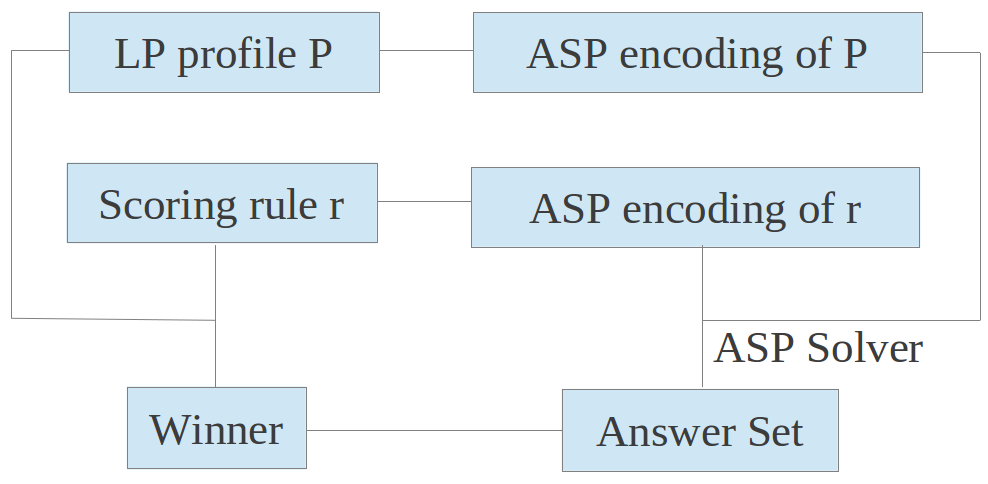
\includegraphics[width=8cm,height=3.8cm]{figs/LPTrees/asp_win_struct.png}
		\caption{The winner problem}
	\end{figure}

	\vspace{-0.45cm}

	\begin{itemize}
		\item Solvers: \tit{clingo}\footcitefull{Gebser:clingo}, 
					\tit{clingcon}\footcitefull{Ostrowski:clingcon}
	\end{itemize}
}

\frameT{Modeling the Problems in W-MAXSAT}
{
	\begin{figure}
		\centering
		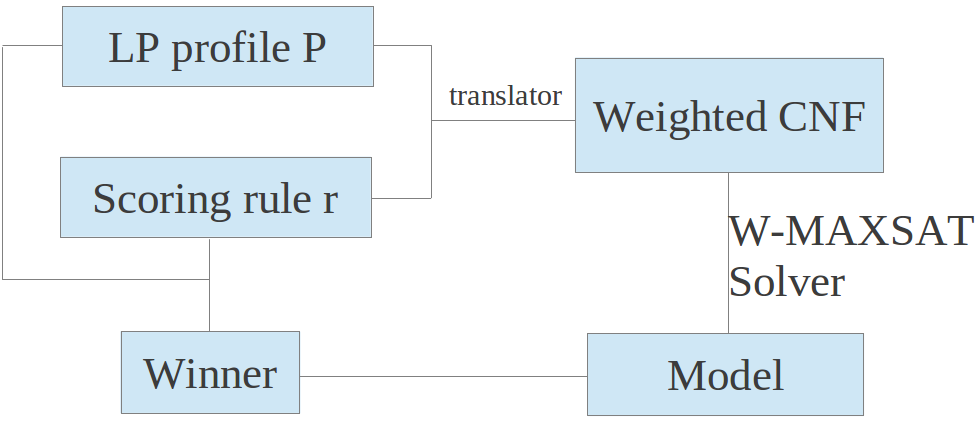
\includegraphics[width=8cm,height=3.6cm]{figs/LPTrees/sat_win_struct.png}
		\caption{The winner problem}
	\end{figure}

	\vspace{-0.45cm}

	\begin{itemize}
		\item Solver: \tit{toulbar}\footcitefull{sanchez2008max}
	\end{itemize}
}

%\frameT{Random LP Profiles}
%{
%	\begin{itemize}
%		\item To experiment with LP profiles, we developed methods to randomly generate
%					\tit{encodings} of
%          a special type of CI-CP LP-tree of size linear in the number of
%          attributes
%	\end{itemize}
%
%	\begin{figure}
%		\vspace{-0.2cm}
%		\centering
%		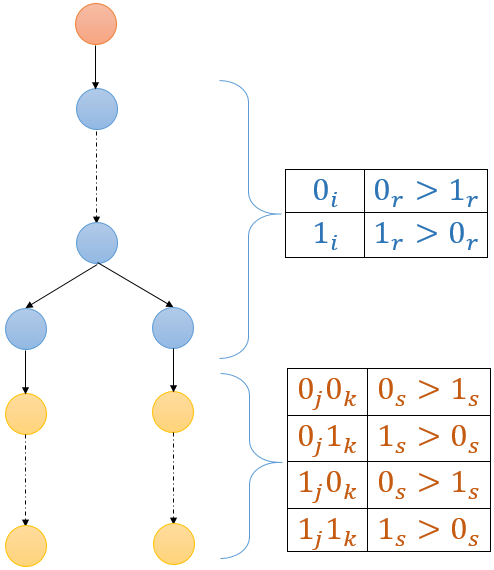
\includegraphics[width=0.4\textwidth]{figs/LPTrees/simple_LP_tree.png}
%		\vspace{-0.3cm}
%		\caption{Random LP-tree}
%	\end{figure}
%}

\frameT{Varying $p$ and $n$: $2^{p-2}$-approval}
{
	\begin{figure}
		\centering
    \begin{subfigure}[b]{0.45\textwidth}
			\centering
			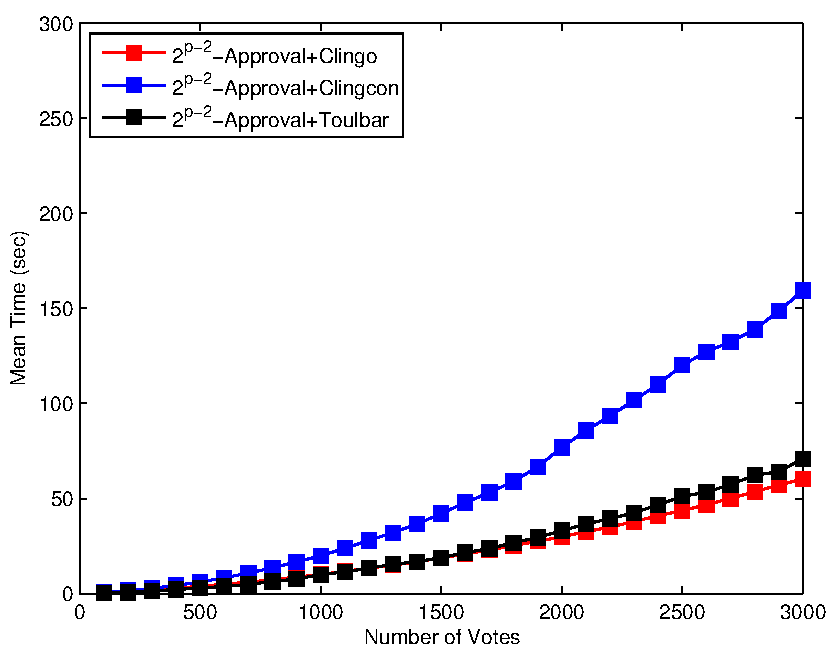
\includegraphics[width=0.95\textwidth]{figs/LPTrees/win/expAppFISCICP.pdf}
			\caption{Fixed \#attributes (10)}
		\end{subfigure}
    \begin{subfigure}[b]{0.45\textwidth}
			\centering
			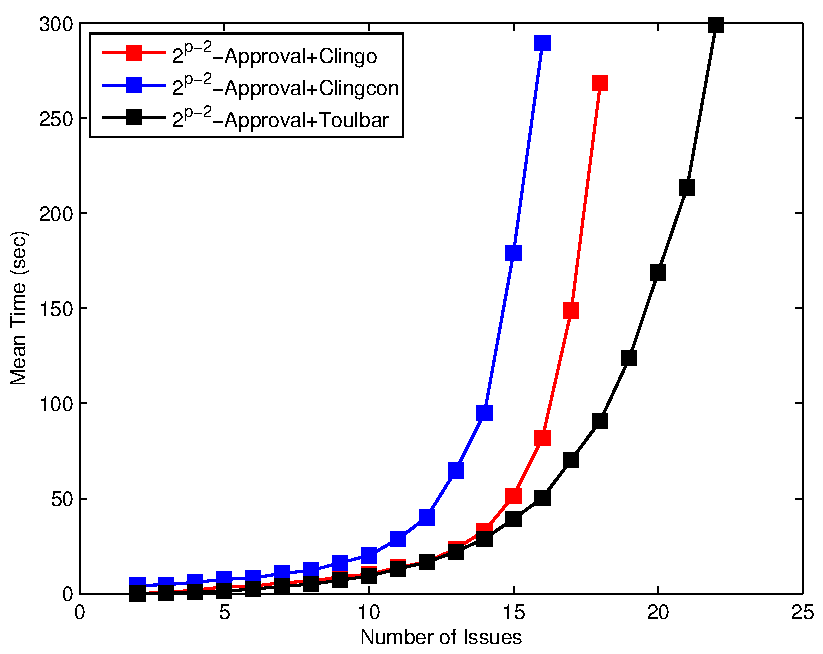
\includegraphics[width=0.95\textwidth]{figs/LPTrees/win/expAppFVSCICP.pdf}
			\caption{Fixed \#votes (1000)}
		\end{subfigure}

		\caption{Solving the winner problem}
	\end{figure}
}

\frameT{Varying $p$ and $n$: ($2^{p-2},2^{p-2}$)-approval
	\fn{
		scoring vector: ($2,\ldots,2,1,\ldots,1,0,\ldots,0$) with the numbers
		of 2's and 1's equal to $2^{p-2}$
	}}
{
	\begin{figure}
		\centering
    \begin{subfigure}[b]{0.45\textwidth}
			\centering
			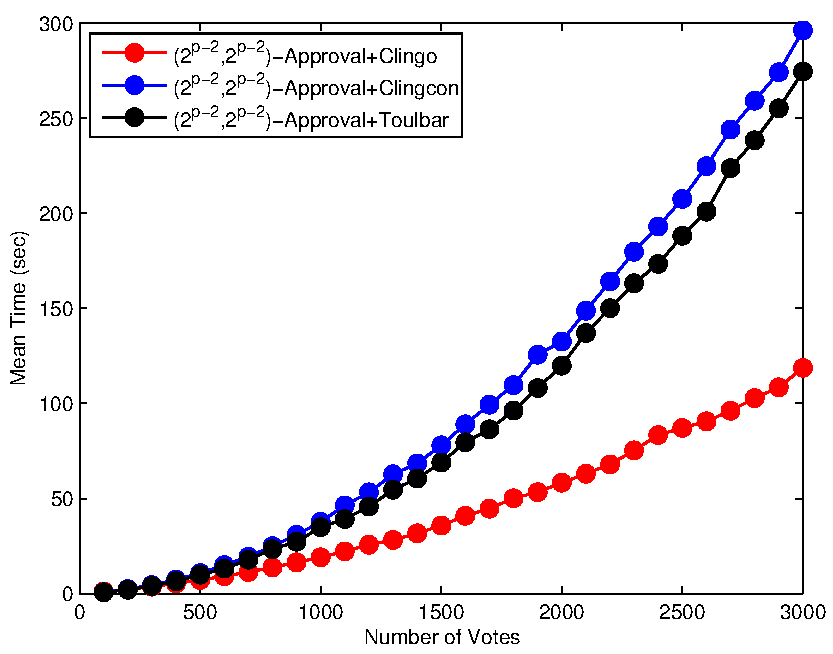
\includegraphics[width=0.95\textwidth]{figs/LPTrees/win/2kAppFISCICP.pdf}
			\caption{Fixed \#attributes (10)}
		\end{subfigure}
    \begin{subfigure}[b]{0.45\textwidth}
			\centering
			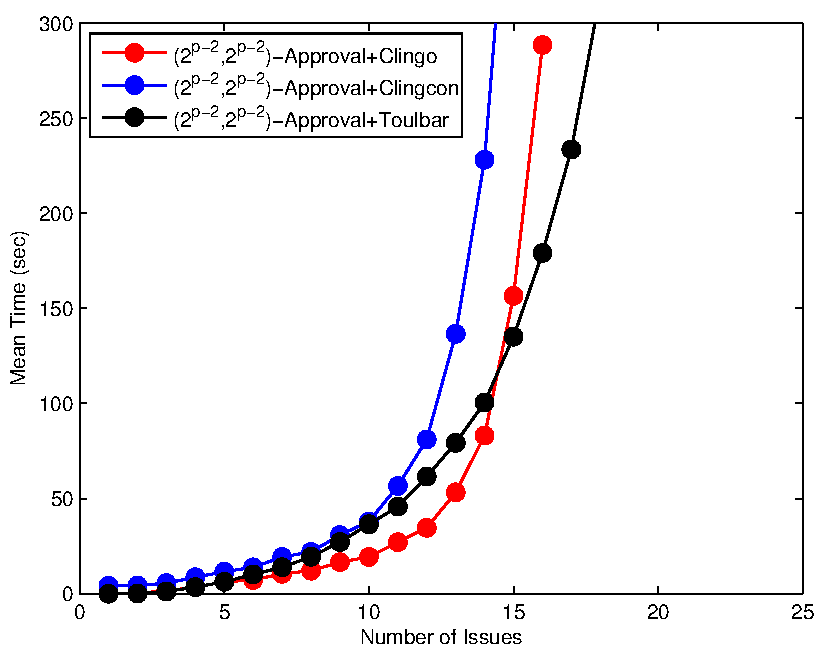
\includegraphics[width=0.95\textwidth]{figs/LPTrees/win/2kAppFVSCICP.pdf}
			\caption{Fixed \#votes (1000)}
		\end{subfigure}
		\caption{Solving the winner problem}
	\end{figure}
}

\frameT{Varying $p$ and $n$: Borda}
{
	\begin{figure}
		\centering
    \begin{subfigure}[b]{0.45\textwidth}
			\centering
			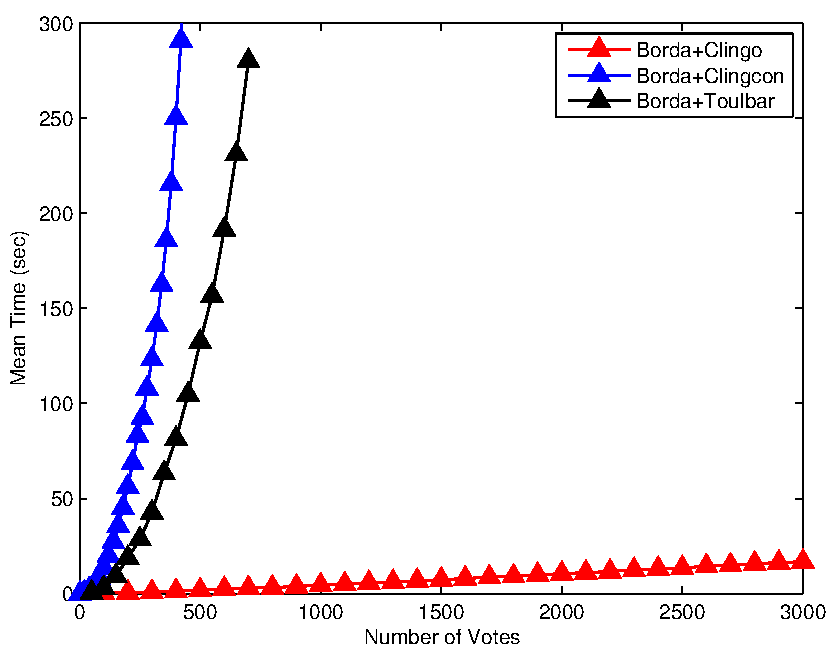
\includegraphics[width=0.95\textwidth]{figs/LPTrees/win/bordaFISCICP.pdf}
			\caption{Fixed \#attributes (10)}
		\end{subfigure}
    \begin{subfigure}[b]{0.45\textwidth}
			\centering
			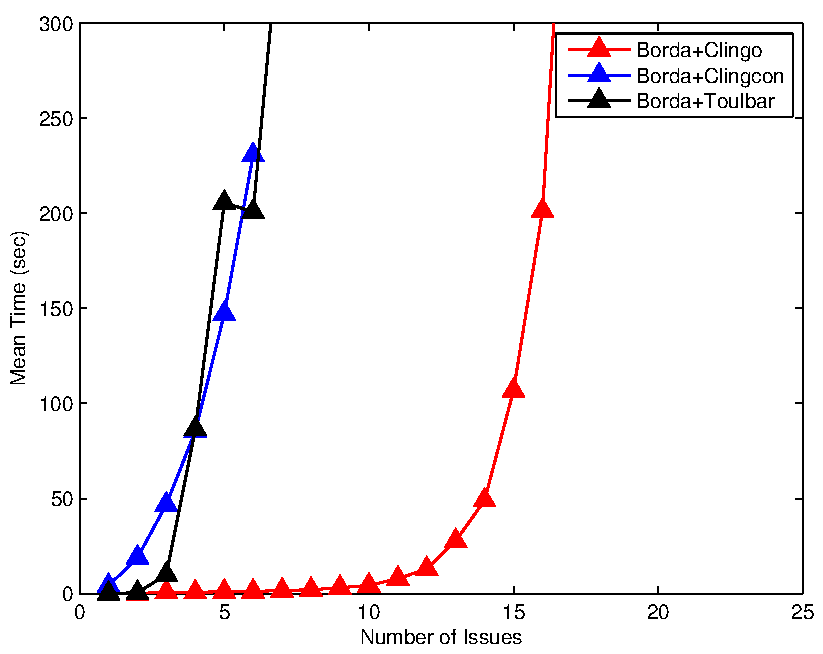
\includegraphics[width=0.95\textwidth]{figs/LPTrees/win/bordaFVSCICP.pdf}
			\caption{Fixed \#votes (1000)}
		\end{subfigure}

		\caption{Solving the winner problem}
	\end{figure}
}

\frameT{Outline}{
  \begin{enumerate}
    {\transparent{0.2} \item The languages of PLP-trees and LP-trees}
    {\transparent{0.2} \item Learning preference models in case of PLP-trees}
    \item Reasoning with preferences:
      \begin{itemize}
        {\transparent{0.2} \item Computing winners and ``strong" candidates when votes are LP-trees}
        \item Application in trip planning
      \end{itemize}
    {\transparent{0.2} \item Future research directions}
  \end{enumerate}
}

\frameT{Personalization in Trip Planning}{
	\begin{enumerate}
		\item Important to incorporate user constraints and preferences into trip
					planning systems.
		\item Collaboration with experts (in AI, planning, optimization, multi-agent systems) at PARC.
		\item Developed a hipergraph-based trip planner that accommodates constraints specified as
					\tit{linear temporal logic} and preferences expressed as \tit{preferential cost function} 
					to compute optimal routes using A*\footcitefull{abs/parc/Liu2}.
		\item Available later for trip planning in the Bay Area, LA, and Denver.
	\end{enumerate}
}

\frameT{Personalization in Trip Planning}{
	\begin{enumerate}
		\item From SJC, to Pier 39, Monday, 9am.
		\item Constraints: never drive a car, and bike for 1 to 2 hours.
		\item Preferences: bike = public (0.25) $>$ wait(2) $>$ walk(3), and 30\$/hr.
	\end{enumerate}

	\vspace{-0.3cm}

	\begin{figure}[ht!]
	  \centering
	    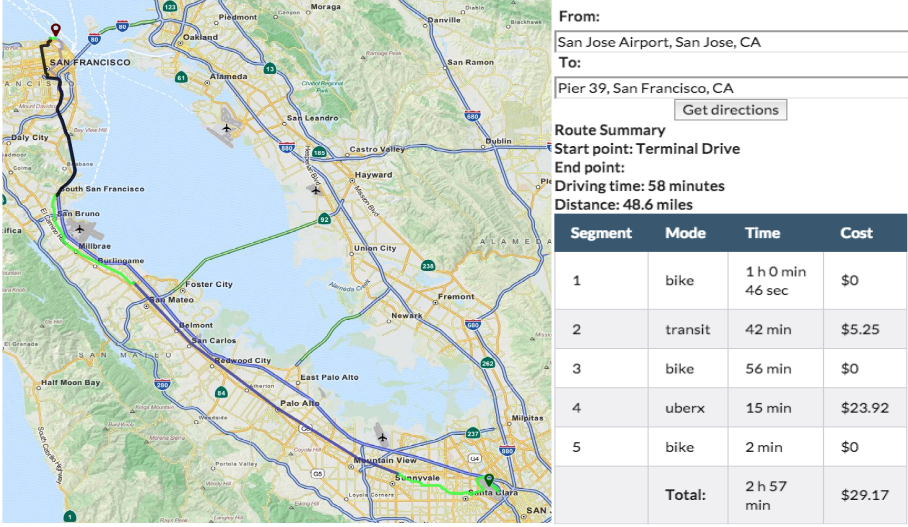
\includegraphics[width=0.7\textwidth]{figs/PARC/route.png}
	\end{figure}
}
